\subsection{Design criteria} \label{ramp_desCrit}
\begin{center}
\begin{tabular}{lp{9cm}}
  \textbf{Materials} & Concrete: f'$_c$ = 4.0 ksi\\
  & Reinforcing steel: f$_y$ = 60 ksi \\
  \textbf{Structural loads} & Self weight reinforced concrete: 2500 $kg/m^3$\\
  & Live load garages (passenger vehicles): 40 psf \\
  & Concentrated load vehicle : 3000 pound \\
  \textbf{Load cases} & D: dead load (see fig. \ref{ramp_D}) \\
  & Lunif: uniform live load (see fig. \ref{ramp_Lunif}) \\
  & LconcSpan1: concentrated live load on mid-span 1 (see fig. \ref{ramp_LconcSpan1}) \\
  & LconcSpan2: concentrated live load on mid-span 2 (see fig. \ref{ramp_LconcSpan2}) \\
  & LconcSpan3: concentrated live load on mid-span 3 (see fig. \ref{ramp_LconcSpan3}) \\
  \textbf{Ultim. Limit States} & ULS01: 1.4*D \\
  & ULS02: 1.2*D + 1.6*Lunif \\
  & ULS03: 1.2*D + 1.6*LconcSpan1 \\
  & ULS04: 1.2*D + 1.6*LconcSpan2 \\
  & ULS05: 1.2*D + 1.6*LconcSpan3 \\
 
  \textbf{Structural model} & 3D elastic computer model (see fig. \ref{ramp_model}) analyzed using XC \\
\end{tabular}
\end{center}

\subsection{Acceptance criteria}
Figure \ref{ramp_reinf} shows the design thickness of the ramp slab and the reinforcing layout.

The slab is checked for the load combinations summarized in section \ref{ramp_desCrit}. The limit state checking was performed in general compliance with ACI 318, using the program XC. The representative plots for the results obtained are shown in figs. \ref{ramp_CF_normal_long} to \ref{ramp_CF_normal_long} for the normal stresses check, and figs. \ref{ramp_CF_shear_long} to \ref{ramp_Vy_shear_trans} for the shear check.
In every case, all the elements have a demand to capacity ratio of 1.0 or less.
\begin{Figure}
    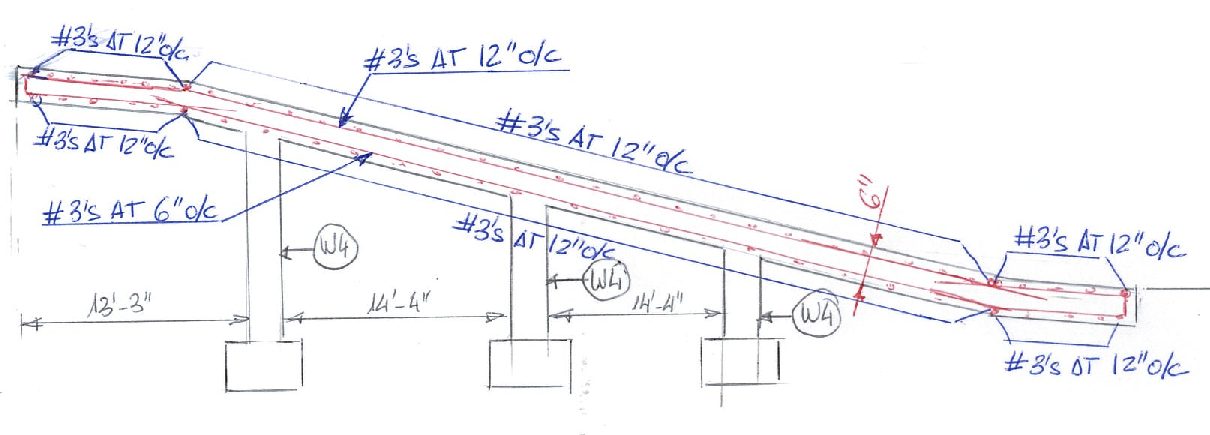
\includegraphics[width=\linewidth]{ramp/figures/ramp_reinf}
    \captionof{figure}{Ramp. Reinforcing layout.}
    \label{ramp_reinf}
\end{Figure}

\twocolumn
\begin{Figure}
    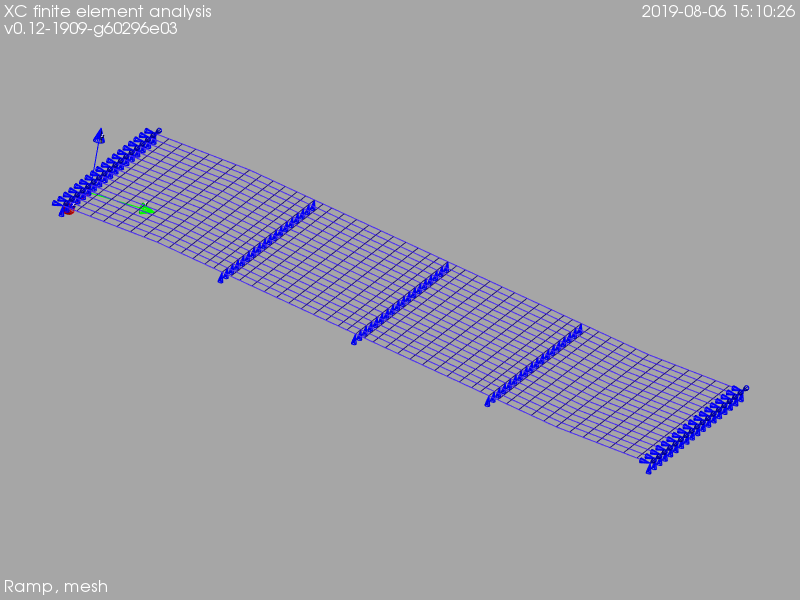
\includegraphics[width=\linewidth]{ramp/figures/ramp}
    \captionof{figure}{Ramp elastic model, mesh.}
    \label{ramp_model}
\end{Figure}
\begin{Figure}
    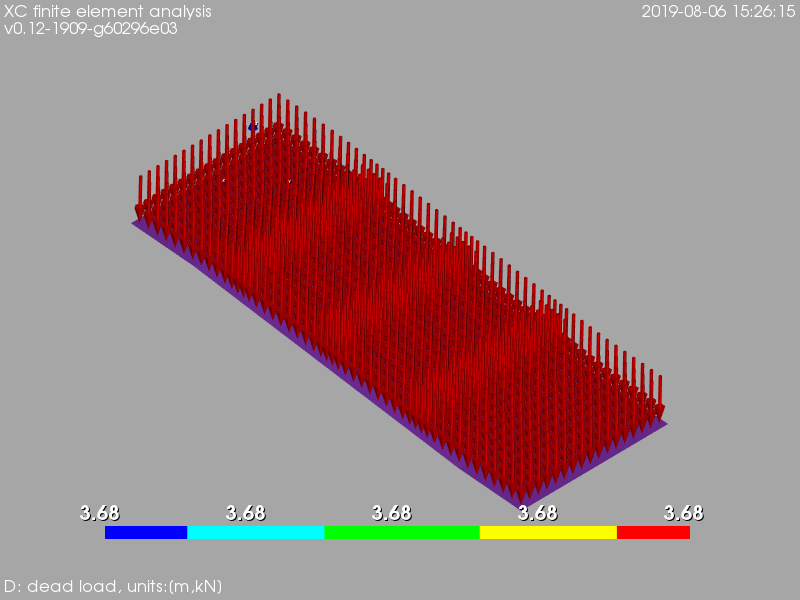
\includegraphics[width=\linewidth]{ramp/figures/D}
    \captionof{figure}{Load case D: dead load (include slab selfweight) [units: $kN/m^2$].}
    \label{ramp_D}
\end{Figure}
\begin{Figure}
    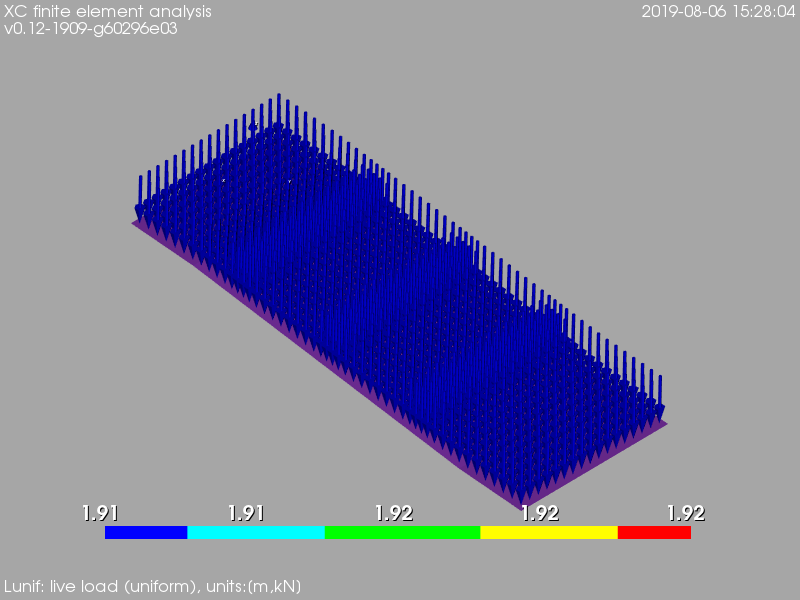
\includegraphics[width=\linewidth]{ramp/figures/Lunif}
    \captionof{figure}{Load case Lv$_{unif}$: uniform live load (vehicles) [units: $kN/m^2$].}
    \label{ramp_Lunif}
\end{Figure}
\begin{Figure}
    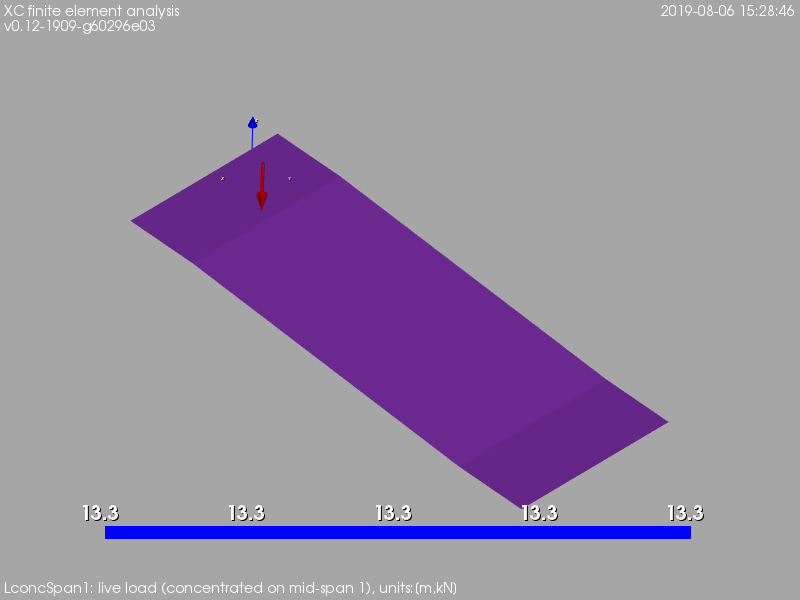
\includegraphics[width=\linewidth]{ramp/figures/LconcSpan1}
    \captionof{figure}{Load case Lv$_{conc,s1}$: concentrated live load (vehicles) on mid-span 1 [units: kN].}
    \label{ramp_LconcSpan1}
\end{Figure}
\begin{Figure}
    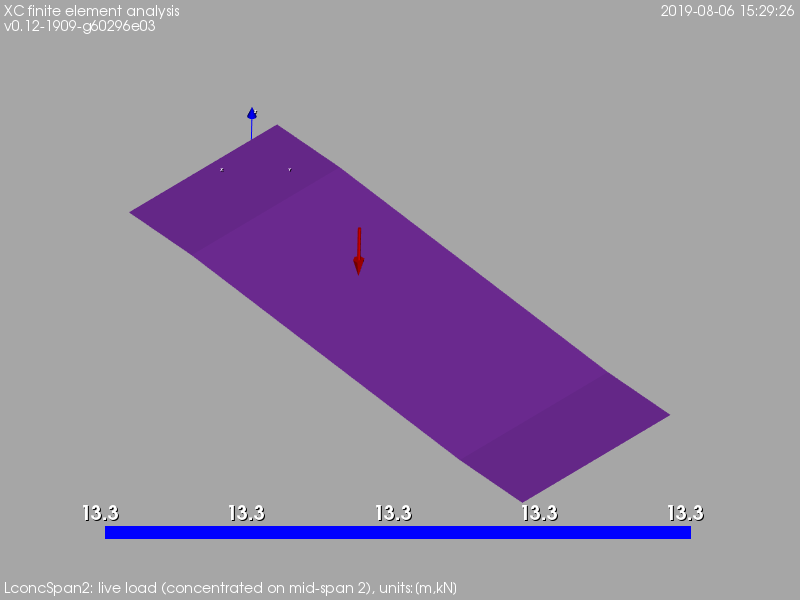
\includegraphics[width=\linewidth]{ramp/figures/LconcSpan2}
    \captionof{figure}{Load case Lv$_{conc,s2}$: concentrated live load (vehicles) on mid-span 2 [units: kN].}
    \label{ramp_LconcSpan2}
\end{Figure}
\begin{Figure}
    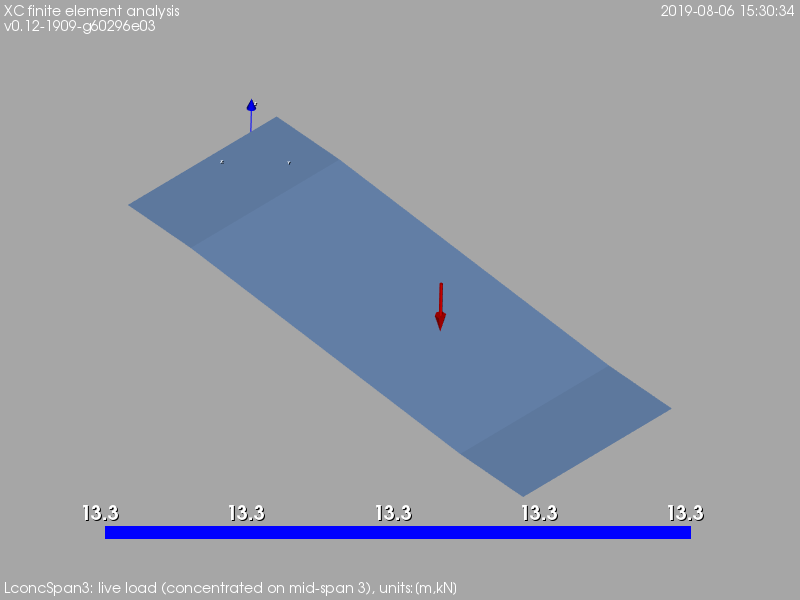
\includegraphics[width=\linewidth]{ramp/figures/LconcSpan3}
    \captionof{figure}{Load case Lv$_{conc,s3}$: concentrated live load (vehicles) on mid-span 3 [units: kN].}
    \label{ramp_LconcSpan3}
\end{Figure}

\begin{Figure}
    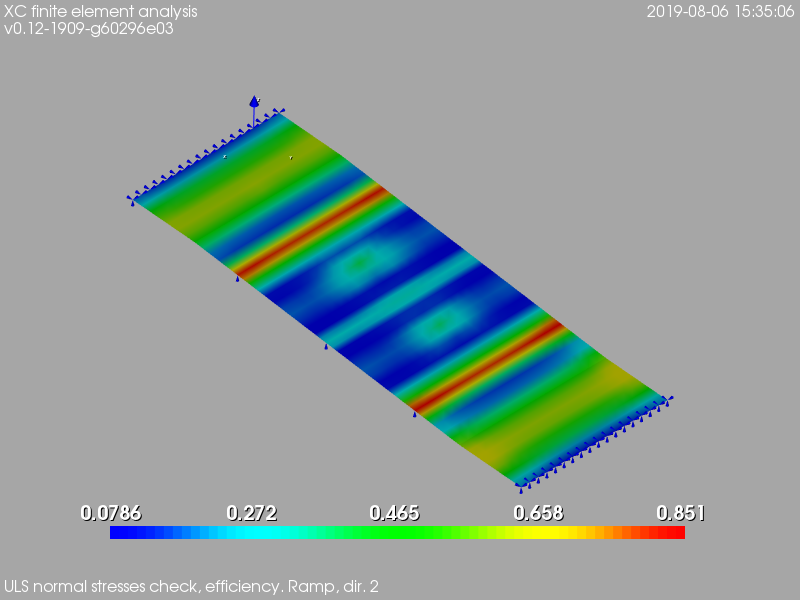
\includegraphics[width=\linewidth]{ramp/figures/CF_normal_long}
    \captionof{figure}{ULS normal stresses check. Efficiency in longitudinal direction}
    \label{ramp_CF_normal_long}
\end{Figure}
\begin{Figure}
    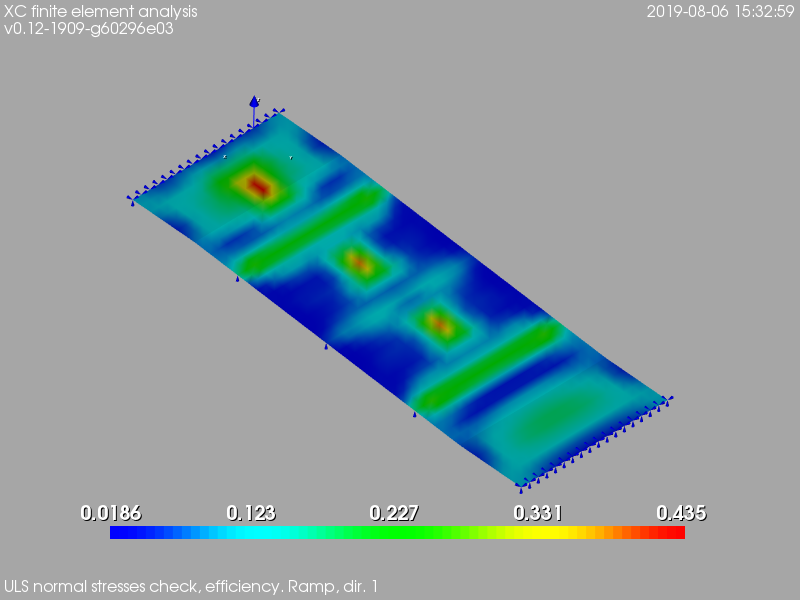
\includegraphics[width=\linewidth]{ramp/figures/CF_normal_trans}
    \captionof{figure}{ULS normal stresses check. Efficiency in transversal direction}
    \label{ramp_CF_normal_trans}
\end{Figure}
\begin{Figure}
    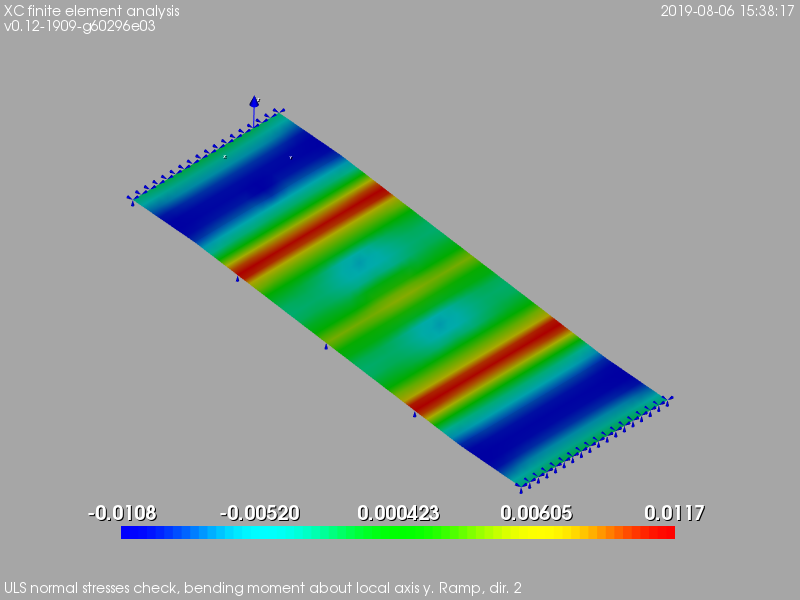
\includegraphics[width=\linewidth]{ramp/figures/My_normal_long}
    \captionof{figure}{ULS normal stresses check. Bending moment in longitudinal direction [units: kN.m].}
    \label{ramp_CF_normal_long}
\end{Figure}
\begin{Figure}
    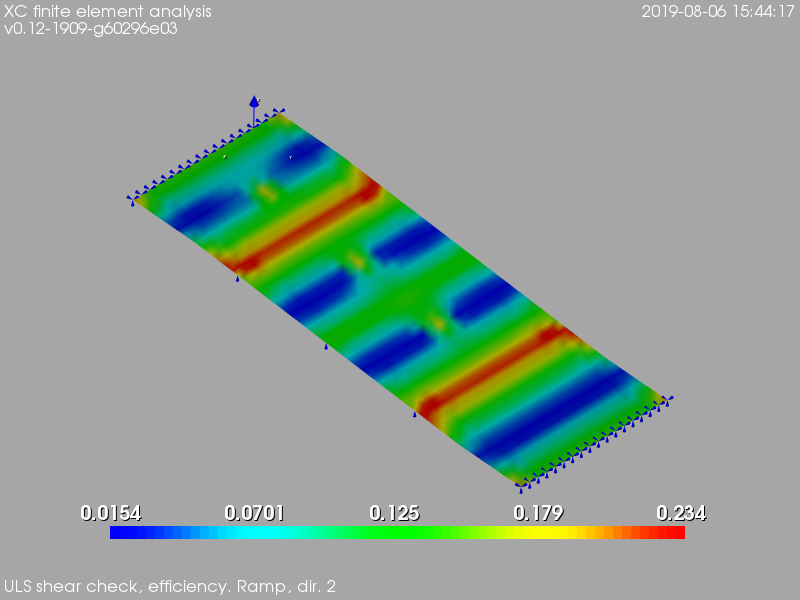
\includegraphics[width=\linewidth]{ramp/figures/CF_shear_long}
    \captionof{figure}{ULS shear check. Efficiency in longitudinal direction}
    \label{ramp_CF_shear_long}
\end{Figure}
\begin{Figure}
    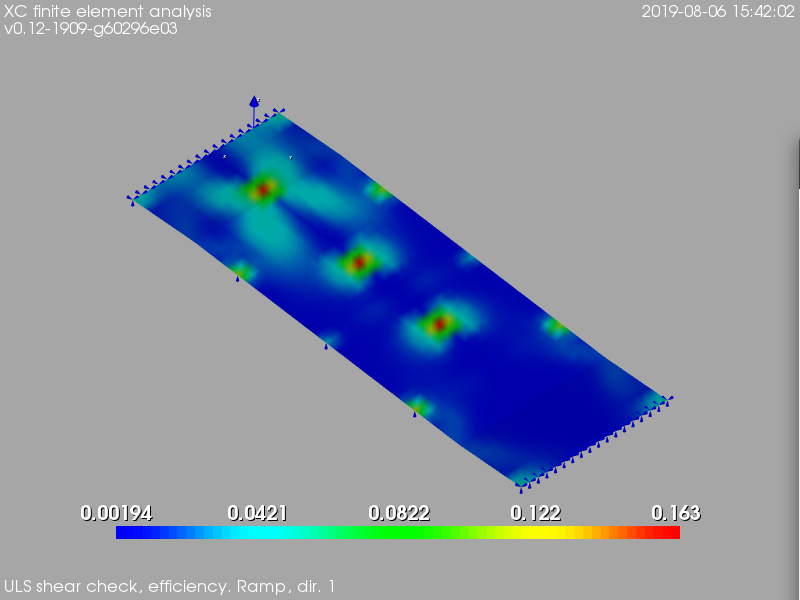
\includegraphics[width=\linewidth]{ramp/figures/CF_shear_trans}
    \captionof{figure}{ULS shear check. Efficiency in transversal direction}
    \label{ramp_CF_shear_trans}
\end{Figure}

\begin{Figure}
    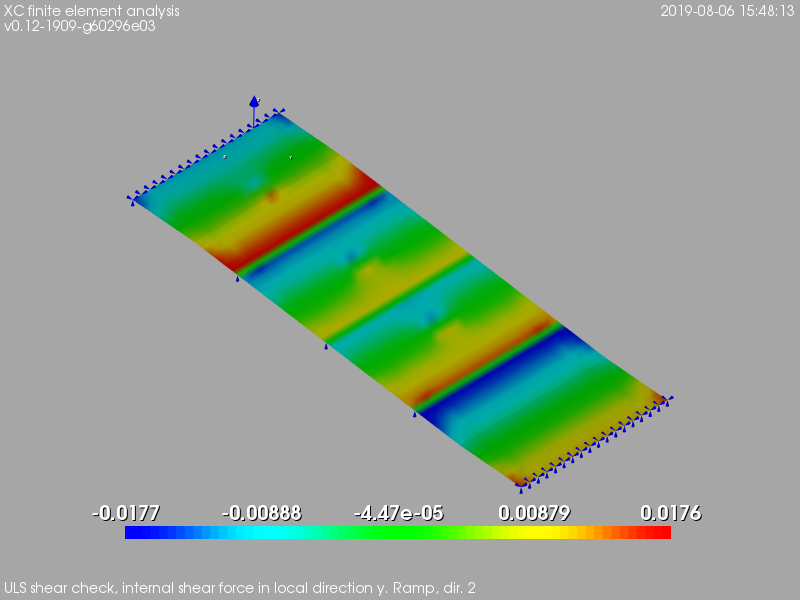
\includegraphics[width=\linewidth]{ramp/figures/Vy_shear_long}
    \captionof{figure}{ULS shear check. Internal shear force in longitudinal direction [units: kN].}
    \label{ramp_Vy_shear_long}
\end{Figure}
\begin{Figure}
    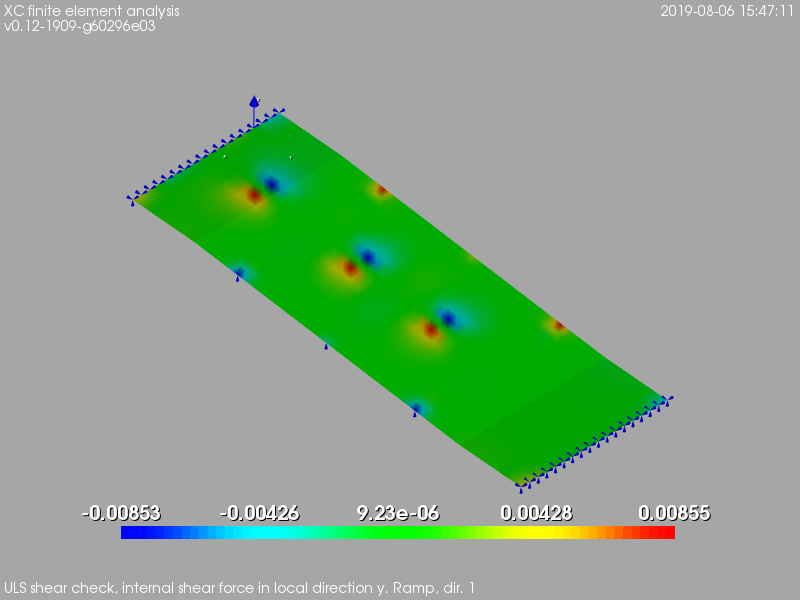
\includegraphics[width=\linewidth]{ramp/figures/Vy_shear_trans}
    \captionof{figure}{ULS shear check. Internal shear force in transversal direction [units: kN].}
    \label{ramp_Vy_shear_trans}
\end{Figure}

\onecolumn

